\chapter{Applicabilità e requisiti tecnici}
\label{chap:applicabilita}
Resta ora da analizzare la fattibilità del progetto nel mondo reale. Questo assistente vocale potrebbe \textbf{migliorare ampiamente il workflow} di molte cliniche ospedaliere, anche all'estero. Infatti, eseguire la traduzione in un'altra lingua è un lavoro svolgibile da chiunque, trattandosi della mera traduzione di stringhe. Si potrebbe, addirittura, pensare di integrare il modulo Python \texttt{googletrans} citato in \ref{section:traduzione}, rendendo il progetto poliglotta.
\section{Requisiti tecnici}
Analizziamo i vari componenti dell'assistente vocale per comprenderne i requisiti tecnici:
\subsection{Text To Speech e Speech To Text}
Queste operazioni vengono svolte in cloud tramite le API di Google, e richiedono quindi \textbf{solamente una connessione ad internet}. Ovviamente, si configura la necessità di periferiche audio per la cattura e la riproduzione di audio. Un \textbf{microfono universale} ed un \textbf{set di altoparlanti} possono sopperire a tale necessità.
\subsection{Analisi degli intent}
L'assistente vocale procede all'analisi degli intent tramite Padatious e Adapt. Mentre il secondo si basa sul riconoscimento di hotwords, e non ha quindi grandi necessità in termini di calcolo, il primo è composto da una rete neurale che viene addestrata ad ogni avvio del bot. Questa è probabilmente l'\textbf{operazione che richiede più potenza} di calcolo. Tuttavia, essendo svolta al solo avvio del bot, basterebbe pensare di avviare il bot \textbf{qualche minuto prima} dell'effettiva necessità di utilizzo per risolvere questa problematica.
\subsection{fastai}
Essendo il training del modello svolto a priori, non avremo grandi necessità di potenza di calcolo: l'operazione di \textit{inference} è \textbf{molto più leggera} dell'addestramento. È suggeribile quindi eseguire quest'ultimo su un computer più potente o direttamente in cloud, con strumenti come Google Colab, per poi \textbf{esportare il modello} nel formato di fastai tramite il comando \texttt{learn.export('/content/exported\_model')}.
\subsection{Interfaccia grafica}
Il software \textbf{Mycroft GUI} fa un pesante utilizzo del framework Qt, più specificatamente dei KDE Plasmoids, componenti grafici (simili a widgets) che caratterizzano l'ambiente desktop KDE Plasma. Per questo, risulta ovvio che il dispositivo su cui viene eseguito l'assistente vocale debba essere compatibile con il suddetto. Il team di Mycroft suggerisce, come sistema operativo, \textbf{KDE neon}, consistente in una versione di  Ubuntu LTS con installato l'ambiente KDE Plasma. Questo nome garantisce un'ottima stabilità, semplicità d'uso, compatibilità.
\section{Compatibilità, dispositivi ottimali e costi}
La sezione precedente ha evidenziato come i requisiti tecnici dell'assistente vocale siano compatibili con una \textbf{vastissima gamma di dispositivi}, anche economici. Questo potrebbe \textbf{sgravare un'ulteriore spesa} ad un sistema ospedaliero vittima, da anni, di tagli e budget stringenti. Il software potrebbe infatti essere installato su un vecchio computer, o su un Raspberry Pi.
\begin{figure}[H]
    \begin{center}
        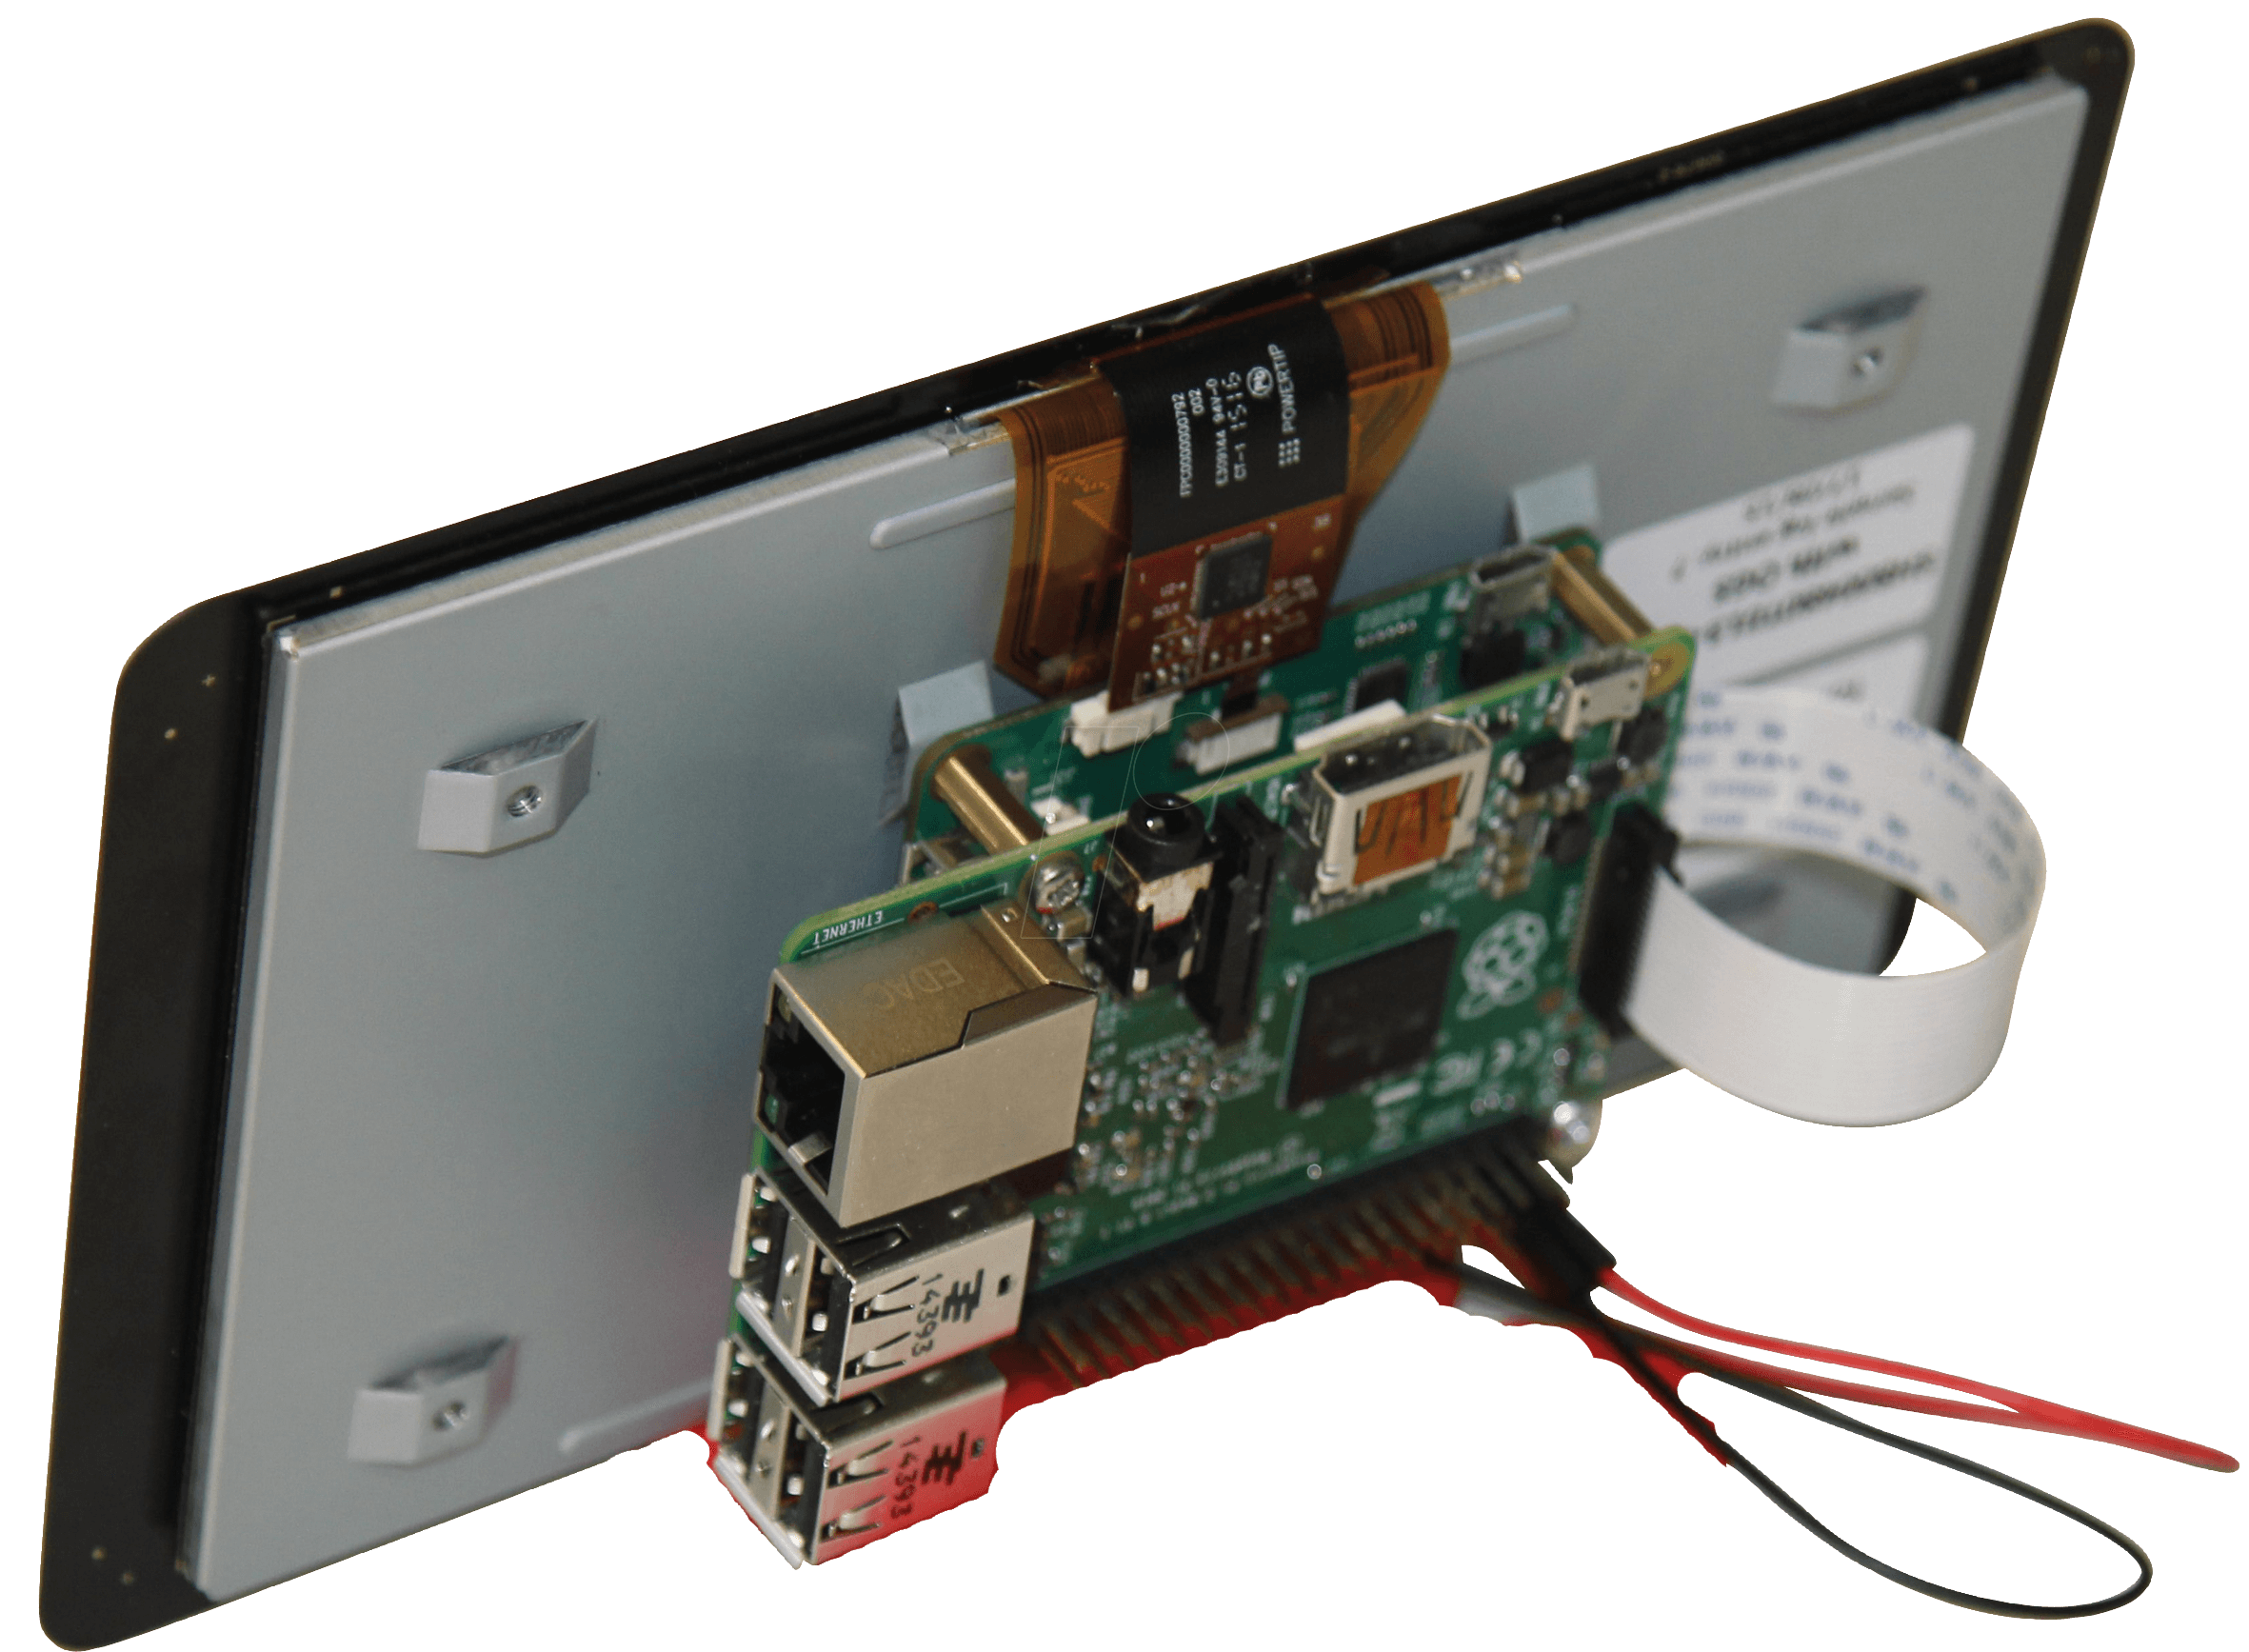
\includegraphics[width=0.8\columnwidth]{images/applicabilita/RPiwithDisplay.png}
    \end{center}
    \caption{Raspberry Pi con display originale}
    \label{fig:raspi-with-display}
\end{figure}
Creando un setup con quest'ultimo, altoparlanti, microfono ed un display da 7", la spesa sarebbe di circa \textbf{cento euro alla data odierna}. Questo costo è senz'altro più basso di tanti dispositivi enterprise proposti ogni giorno agli ospedali, oltre a garantire \textbf{tutela dei dati}, \textbf{apertura delle logiche} di funzionamento (open source), \textbf{semplicità} di utilizzo. Un altro dispositivo molto interessante per questo progetto è il \textbf{Mycroft Mark II}, sviluppato direttamente dai creatori dell'assistente vocale, integrante tecnologie di cancellazione del rumore, un display per l'interfaccia grafica, altoparlanti e kernel Linux, con possibilità di accesso SSH per la configurazione e la codifica di nuove skills. Quest'ultimo costerà, al suo lancio, poco più di cento euro, e rappresenta l'alternativa perfetta ad un sistema autocostruito, probabilmente troppo sperimentale per un ospedale. La \textbf{privacy} è in ogni caso \textbf{garantita} dal team.
\begin{figure}[H]
    \begin{center}
        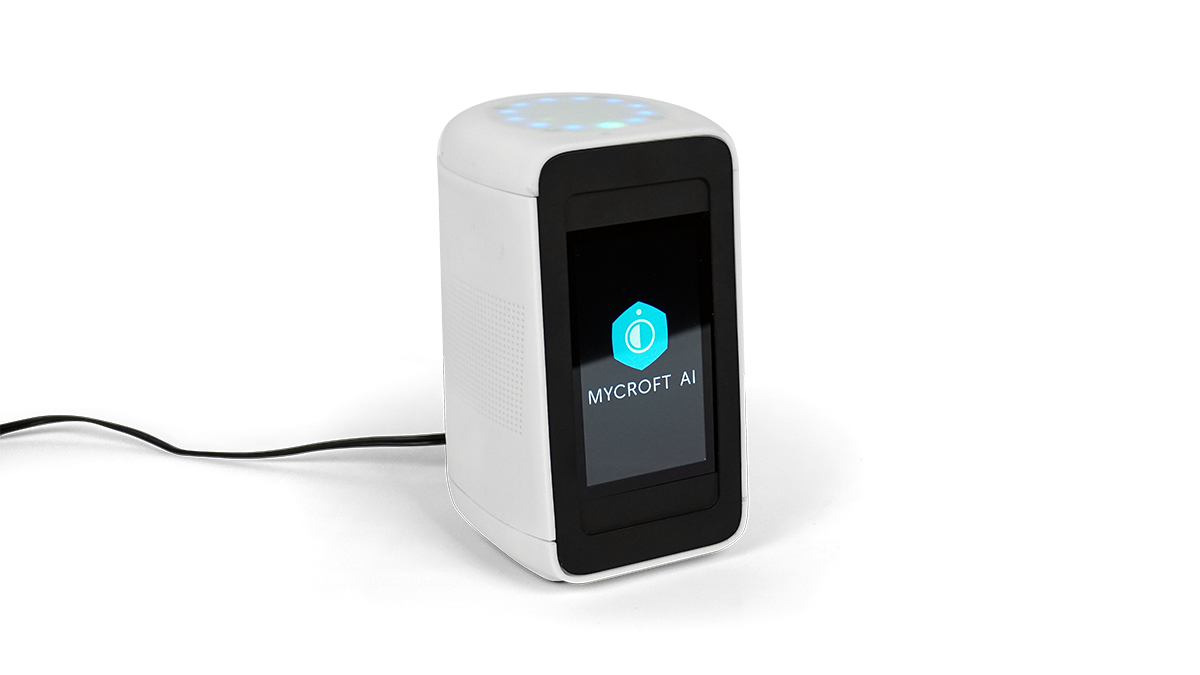
\includegraphics[width=0.8\columnwidth]{images/applicabilita/Mark_II.png}
    \end{center}
    \caption{Mycroft Mark II}
    \label{fig:mark-II}
\end{figure}
\begin{center}
    \textit{The Mycroft Mark II smart speaker is an open solution for individuals and companies who want to deploy voice technology, but don’t want to be in orbit around Silicon Valley.  Our technology can be run on premises and provides a great voice experience without sacrificing privacy.}
\end{center}
